\documentclass[10pt,twocolumn,letterpaper]{article}

\usepackage{cvpr}
\usepackage{times}
\usepackage{epsfig}
\usepackage{graphicx}
\usepackage{amsmath}
\usepackage{amssymb}
\usepackage{float}
\usepackage{listings}
\usepackage{color} %red, green, blue, yellow, cyan, magenta, black, white
\definecolor{mygreen}{RGB}{28,172,0} % color values Red, Green, Blue
\definecolor{mylilas}{RGB}{170,55,241}
\usepackage{subcaption}
\usepackage{booktabs}

% Include other packages here, before hyperref.

% If you comment hyperref and then uncomment it, you should delete
% egpaper.aux before re-running latex.  (Or just hit 'q' on the first latex
% run, let it finish, and you should be clear).
\usepackage[breaklinks=true,bookmarks=false]{hyperref}

\cvprfinalcopy % *** Uncomment this line for the final submission

\def\cvprPaperID{****} % *** Enter the CVPR Paper ID here
\def\httilde{\mbox{\tt\raisebox{-.5ex}{\symbol{126}}}}

% Pages are numbered in submission mode, and unnumbered in camera-ready
%\ifcvprfinal\pagestyle{empty}\fi
\setcounter{page}{1}
\begin{document}

%%%%%%%%% TITLE
\title{Machine Learining for Computer Vision Coursework 2\\
	Visual Categorisation by BoW (K-means) and SVM
	}

\author{David Angelov\\
MEng Electrical and Electronic Engineering \\
Imperial College London\\
{\tt\small david.angelov12@imperial.ac.uk}
% For a paper whose authors are all at the same institution,
% omit the following lines up until the closing ``}''.
% Additional authors and addresses can be added with ``\and'',
% just like the second author.
% To save space, use either the email address or home page, not both
\and
Huaqi Qiu\\
MSc Communication and Signal Processing\\
Imperial College London\\
{\tt\small h.qiu15@imperial.ac.uk}
}

\maketitle
%\thispagestyle{empty}

%%%%%%%%% BODY TEXT
\section{Question 1}

%-------------------------------------------------------------------------
%\begin{figure}[H]
%	\begin{center}
%		\includegraphics[width=0.8\linewidth]{q1_meanface}
%		\caption{Mean face}
%	\end{center}
%	\label{fig:q1_meanface}
%\end{figure}



%------------------------------------------------------------------------
\section{Question 2}

\subsection{Theory of SVM and multi-class extension}
In this coursework, we applied Support Vector Machine (SVM) as the classifier. SVM is a binary classifier based on the discriminant function

\begin{equation}
y(\boldsymbol{x}) = \boldsymbol{w^T x} + b
\label{eq:svm_linear}
\end{equation}

where $\boldsymbol{w}$ is a weight vector and $b$ is the bias. The dataset $x$ is classified to one of the two classes according to the value of $y(\boldsymbol{x})$. However, there are cases when dataset is not linearly separable, in which the Kernel Trick is required. The Kernel Trick map the data points to a higher-dimensional feature space so that the dataset is linearly separable. This process is denoted by: $\boldsymbol{x} \rightarrow \phi (\boldsymbol{x})$. Now the binary SVM function (Eq.\ref{eq:svm_linear}) becomes

\begin{equation}
y(\boldsymbol{x}) = \boldsymbol{w^T} \phi (\boldsymbol{x}) + b
\end{equation}

The SVM separate data in the Kernel transformed space by a linear decision hyperplane. The best hyperplane is found by maximizing the margin of separation. The margin is evaluated by finding the distance of the closest training point to the decision hyperplane. The optimised weighting vector $\boldsymbol{w}$ takes the form of

\begin{equation}
\boldsymbol{w} = \sum_{n=1}^{N} a_n t_n \phi(\boldsymbol{x_n})
\end{equation}

where $\boldsymbol{x_n}$ is training data vector and $t_n$ is the labels of the $n^{th}$ training data vector. Then the SVM decision function becomes

\begin{equation}
	y(\boldsymbol{x}) = \sum_{n=1}^{N} a_n t_n k(\boldsymbol{x}, \boldsymbol{x}_n)  + b
\end{equation}

where $k(\boldsymbol{x}, \boldsymbol{x}_n) $ is the Kernel function. In this course work we primarily consider the RBF kernel function, which is formulated as

\begin{equation}
 k(\boldsymbol{x}, \boldsymbol{x'}) = exp(\frac{||\boldsymbol{x} - \boldsymbol{x'}||^2}{2 \sigma^2})
 \label{eq:RBF}
\end{equation}

We considered the parameter $\sigma$ in the kernel function as the primary factor that affects the performance of RBF kernel SVM. We also considered the parameter $C$, which is an error weighting constant that penalizes the misclassification during the supervised learning and effectively controls the margin.

Since SVM is two-class classifier, we extended it in order to solve multi-class classification problems. Two methods of extension were considered:

\begin{enumerate}
	\item One versus the rest (OVR)\\
	In OVR method, we trained $M$ separate SVMs for $M$ class problem. In the training of the $m^{th}$ SVM, the $m^{th}$ class were labelled as positive class, while the rest $M-1$ classes were labelled as negative class. Upon testing a query image $\boldsymbol{x}$, the output from all $M$ SVMs were compared. The query image was classified as the $m^{th}$ image if the output of the $m^{th}$ SVM was the highest, i.e.
	\begin{equation}
		y(\boldsymbol{x}) = max_m \{ y_m(\boldsymbol{x}) \}
	\end{equation}
	
	\item One versus one (OVO)\\
	In OVO method, we trained SVMs by pairs of the classes. Each of the $M(M-1)/2$ SVMs was trained by data from a pair of two classes, labelling data points from one of the class as the positive class. In testing, the query image was tested and the output from each SVM was treated as 'vote'. The class that had the majority of votes was the class that the query image was classified to.
\end{enumerate}

\subsection{Implementation on Toy Spiral data}
In this coursework, we firstly tested the SVM theory on the Toy Spiral data, shown in Figure~\ref{fig:q2_data}. Each data point is in the form of $ [(X_n, Y_n), t_n]$, where $(X_n, Y_n)$ is 2-D Cartesian coordinates and $t_n$ is the class label of the data point. The testing data is a 2D dense grid within the range of $X_n, Y_n \in [-1.5, 1.5]$. Testing with this testing data set can visualise the decision boundaries.

\begin{figure}
	\begin{center}
		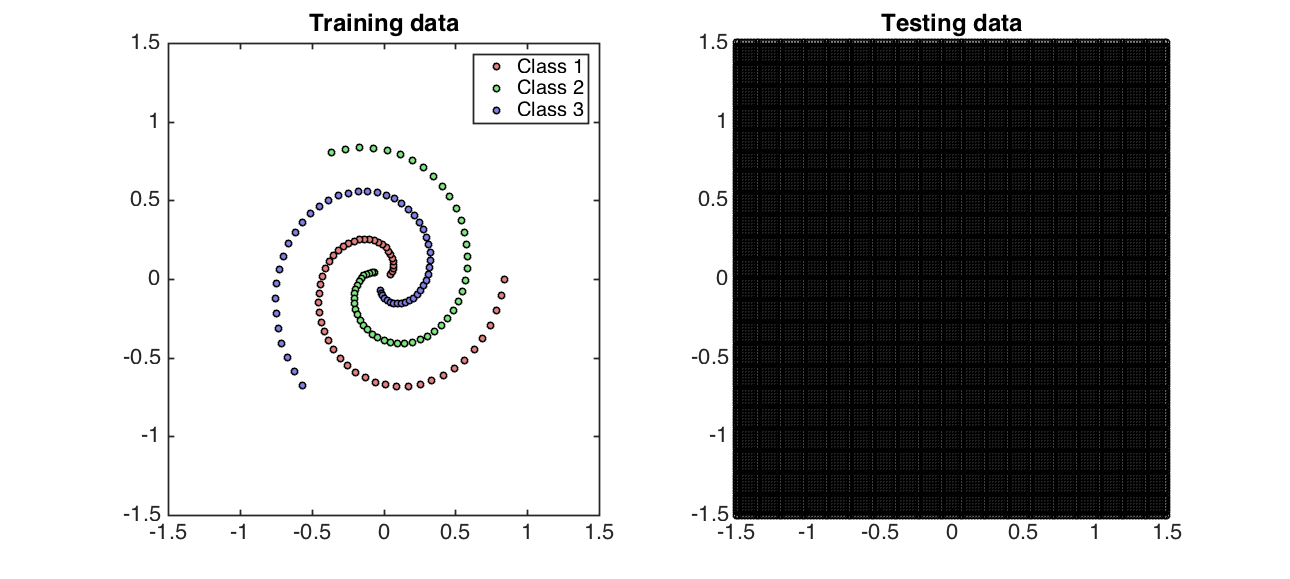
\includegraphics[width=0.8\linewidth]{q2_data}
		\caption{Toy Spiral training and testing data face}
			\label{fig:q2_data}
	\end{center}
\end{figure}

\subsection{SVM extension}
As introduced previously, we extended the binary class SVMs to multi-class SVMs by OVR and OVO. Figure~\ref{fig:q2_ovr_3} shows the classification results from each of the 3 SVMs extended by OVR method. In this Figure, red regions represents the positive class classified by the SVM. The combined classification of the 3 SVMs is shown in Figure~\ref{fig:q2_ovr}. In all demonstrations in this part of the discussion, the kernel coefficients $\sigma$ and $C$ are kept unchanged ($\sigma = 0.8$ and $C = \infty$).

\begin{figure}
	\begin{center}
		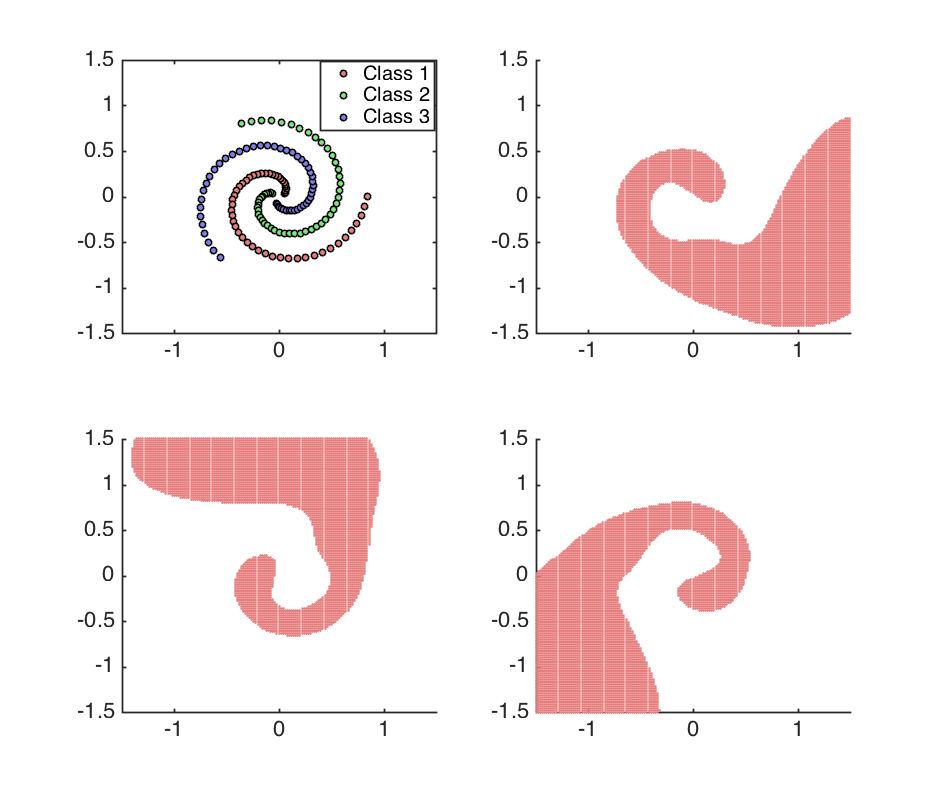
\includegraphics[width=0.8\linewidth]{q2_ovr_3}
		\caption{Result form each OVR extended SVMs}
		\label{fig:q2_ovr_3}
	\end{center}
\end{figure}

\begin{figure}
	\begin{center}
		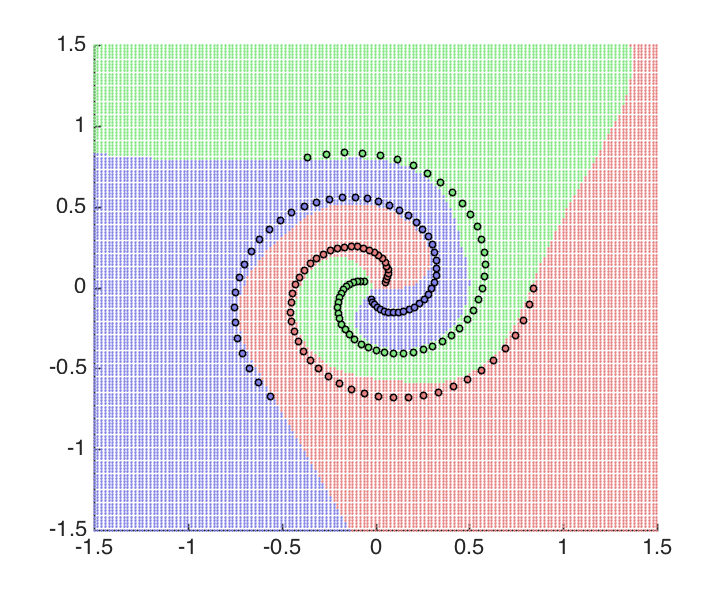
\includegraphics[width=0.8\linewidth]{q2_ovr_sig08}
		\caption{Combined result of OVR extended SVMs}
		\label{fig:q2_ovr}
	\end{center}
\end{figure}

Similarly, Figure~\ref{fig:q2_ovo_3} and~\ref{fig:q2_ovo} show the results of individual SVMs and their combination respectively. Notice that in the OVO case, the votes from all $M(M-1)$ might not have a single majority. Data points with these classification results were classified as 0 in this question, which corresponds to the 'white' area in Figure~\ref{fig:q2_ovo}. For the recognition problem of Caltech 101 data in question 4, we randomly selected class labels from all classes for these type of data points by \texttt{randi}. 

\begin{figure}
	\begin{center}
		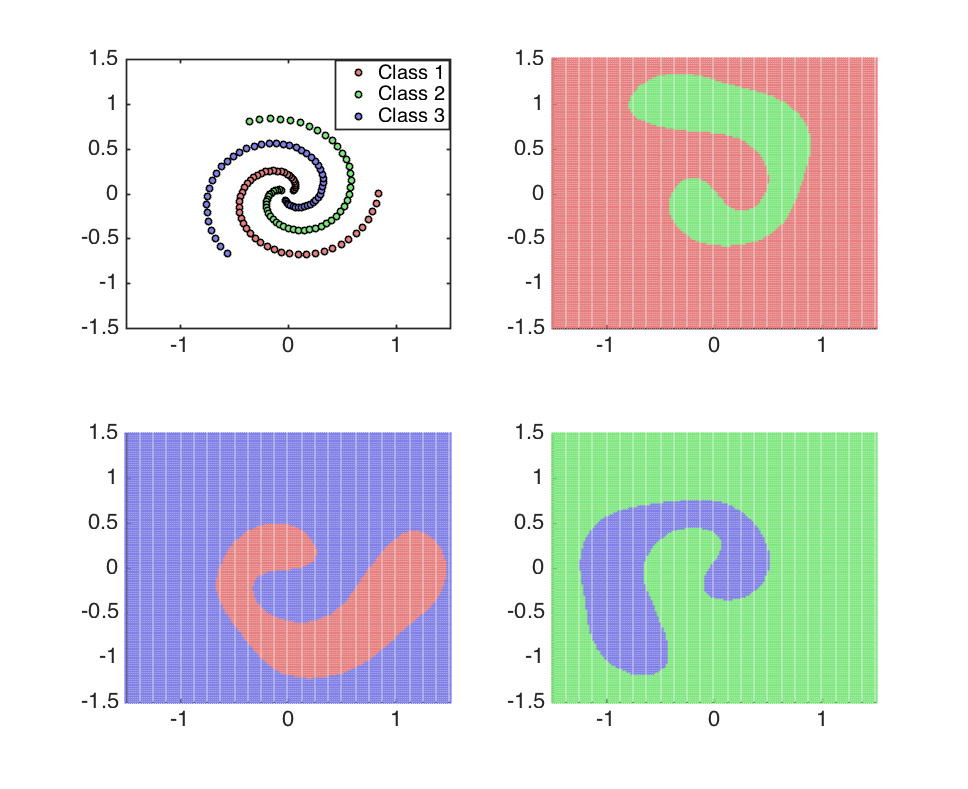
\includegraphics[width=0.8\linewidth]{q2_ovo_3}
		\caption{Result form each OVO extended SVMs}
		\label{fig:q2_ovo_3}
	\end{center}
\end{figure}

\begin{figure}
	\begin{center}
		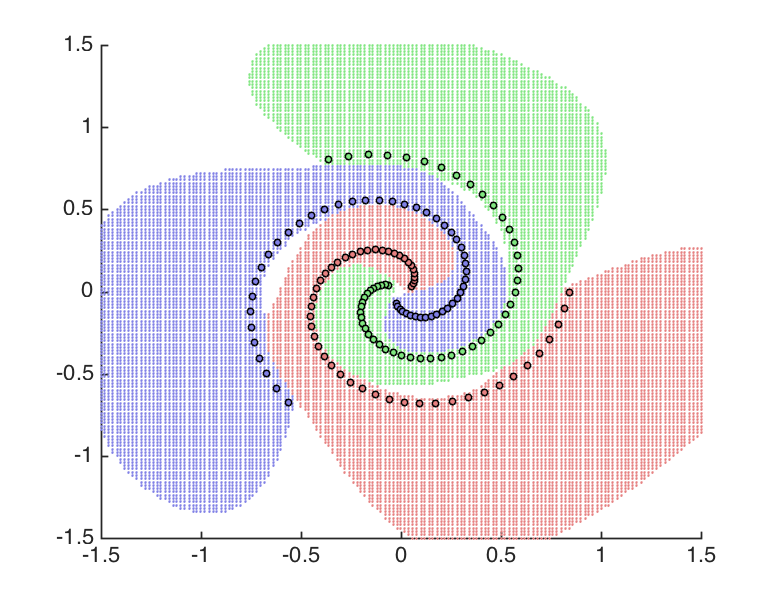
\includegraphics[width=0.8\linewidth]{q2_ovo}
		\caption{Combined result of OVO extended SVMs}
		\label{fig:q2_ovo}
	\end{center}
\end{figure}

\subsection{SVM parameters}
The parameters $\sigma$ for the RBF kernel function and the parameter $C$ for the misclassification penalty are problem dependent. Here we discuss the effect of the two parameters using the Toy Spiral data test. The kernel parameter $\sigma$ affects the generalization or complexity of the model. Simpler models could have better generalization to unseen data with the risk of underfitting. Complex models on the other hand could be overfitted to training data and results in high testing loss (i.e. lower classification accuracy). This can be reflected on the fact that the more complex the system gets, the more support vectors are utilised to construct the marginal boundaries. Figure (a), (b) and (c) in Figure~\ref{fig:q2_ovr_all} show the result of varying the parameter $\sigma$ while keeping $C$ unchanged. Result (a) demonstrates the case of overfitting and (c) demonstrates the case of underfitting.

The parameter $C$ for each misclassified data point is proportional to its distance from the decision boundary. This indicates that $C$ controls the margin allowed for the SVMs. The plots (d), (e) and (f) in FIgure~\ref{fig:q2_ovr_all} present the classification results of varying the parameter $C$ while keeping $\sigma$ unchanged. The result of (d) suggests that the model was underfitting when $C$ is low, while (e) and (f) indicate that the performance of the model could converges when $C$ is sufficiently large. We will further discuss the effects of the parameters $\sigma$ and $C$ in a numerical manner (accuracy) for the Caltech101 data set. 

\begin{figure}

\begin{subfigure}[H]{0.3 \columnwidth}
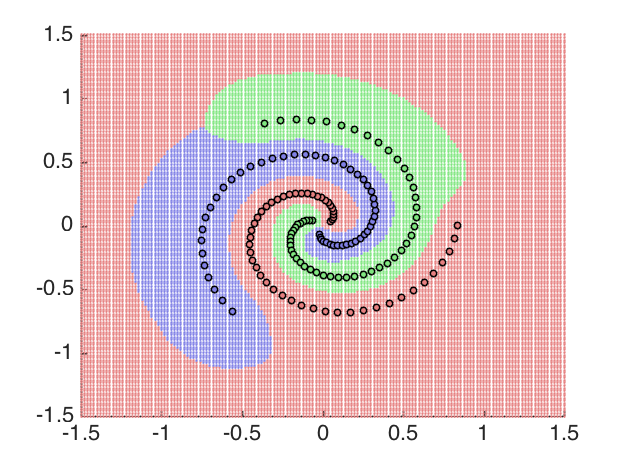
\includegraphics[width = 1\columnwidth]{q2_ovr_sig02}\hfill
\caption{$\sigma = 0.2$}
\end{subfigure}
~
\begin{subfigure}[H]{0.3 \columnwidth}
	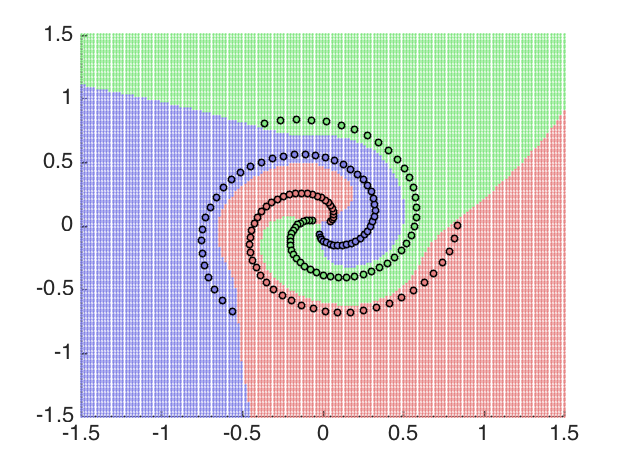
\includegraphics[width = 1\columnwidth]{q2_ovr_sig1}
	\caption{$\sigma = 1$}
\end{subfigure}
~
\begin{subfigure}[H]{0.3 \columnwidth}
	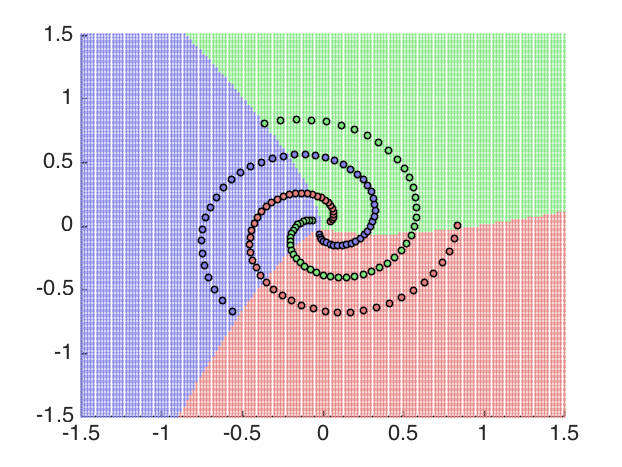
\includegraphics[width = 1\columnwidth]{q2_ovr_sig5}
	\caption{$\sigma = 5$}
\end{subfigure}

	\begin{subfigure}[H]{0.3 \columnwidth}
		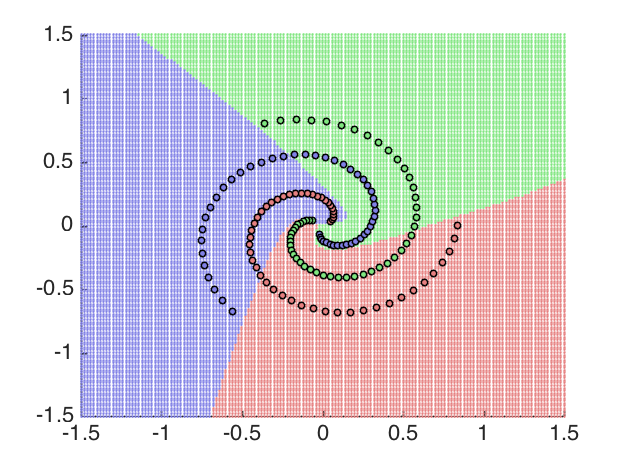
\includegraphics[width = 1\columnwidth]{q2_ovr_C1}\hfill
		\caption{$C = 1$}
	\end{subfigure}
	~
	\begin{subfigure}[H]{0.3 \columnwidth}
		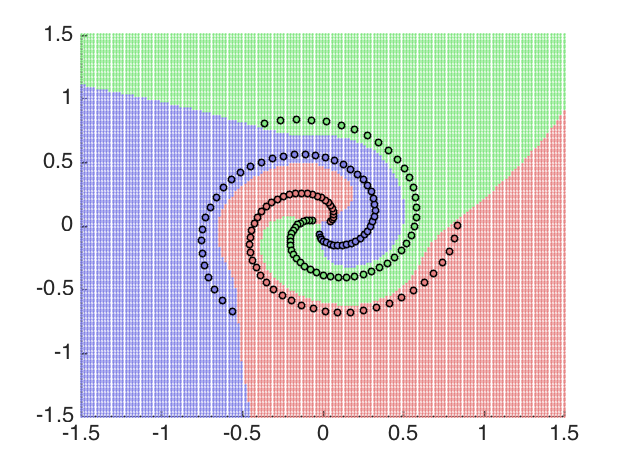
\includegraphics[width = 1\columnwidth]{q2_ovr_C1000}
		\caption{$C = 1000$}
	\end{subfigure}
	~
	\begin{subfigure}[H]{0.3 \columnwidth}
		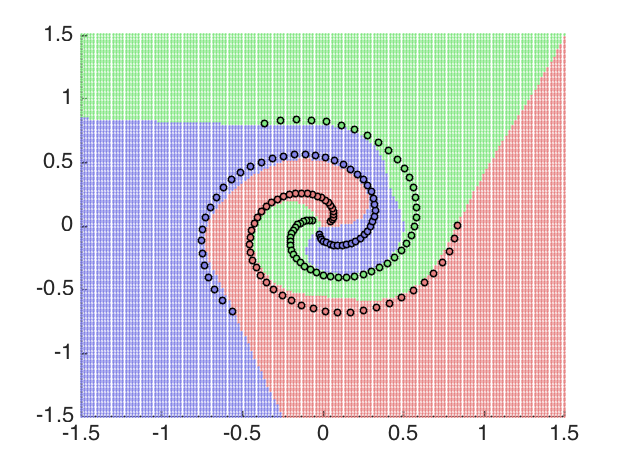
\includegraphics[width = 1\columnwidth]{q2_ovr_Cinf}
		\caption{$C = \infty$}
	\end{subfigure}
	
	\caption{Classification results with varying parameters $\sigma$ and $C$ for OVR}
	\label{fig:q2_ovr_all}
\end{figure}



\section{Question 3}
In this question, we performed image recognition using the Caltech101 data set. We randomly selected 15 images from each of the 10 different classes. The performance of the classification was evaluated by the correction rate of image classification. We investigated the following parameters that could affect the accuracy:

\begin{itemize}
	\item Vocabulary size = $K$
	\item Kernel types (RBF and Polynomial) and kernel parameters ($\sigma$ for RBF, polynomial order $M$ for polynomial)
	\item Misclassification penalty parameter $C$
\end{itemize}


\subsection{Bag of Words}
Both training and testing images are transformed into data points for classification by the Bag-of-Words technique, which utilized the K-means clustering in Question 1. This process can be described as:

\begin{enumerate}
 \item Visual vocabulary construction (using K-means clustering)\\
 We firstly apply the Scale Invariant Feature Transform (SIFT) descriptor to extract features (visual words) from each image. Each SIFT descriptor $\boldsymbol{d}$ has a dimension of $D = 128$. Then, we selected 100,000 descriptors and applied the K-means clustering. The K cluster centres found are called codewords or visual vocabulary.

\item Histogram of visual words\\
Each image was represented by a histogram of visual words, which is constructed by assigning the visual words to the codewords by the Nearest Neighbour matching and counting the number of words assigned to each codeword. The distance between visual words and codewords can be evaluated by the Euclidean distance, i.e.

\begin{equation}
 E(\boldsymbol{d_1}, \boldsymbol{d_2}) = || \boldsymbol{d_1} - \boldsymbol{d_2}||
\end{equation}
\end{enumerate}


\begin{figure}
	\begin{center}
		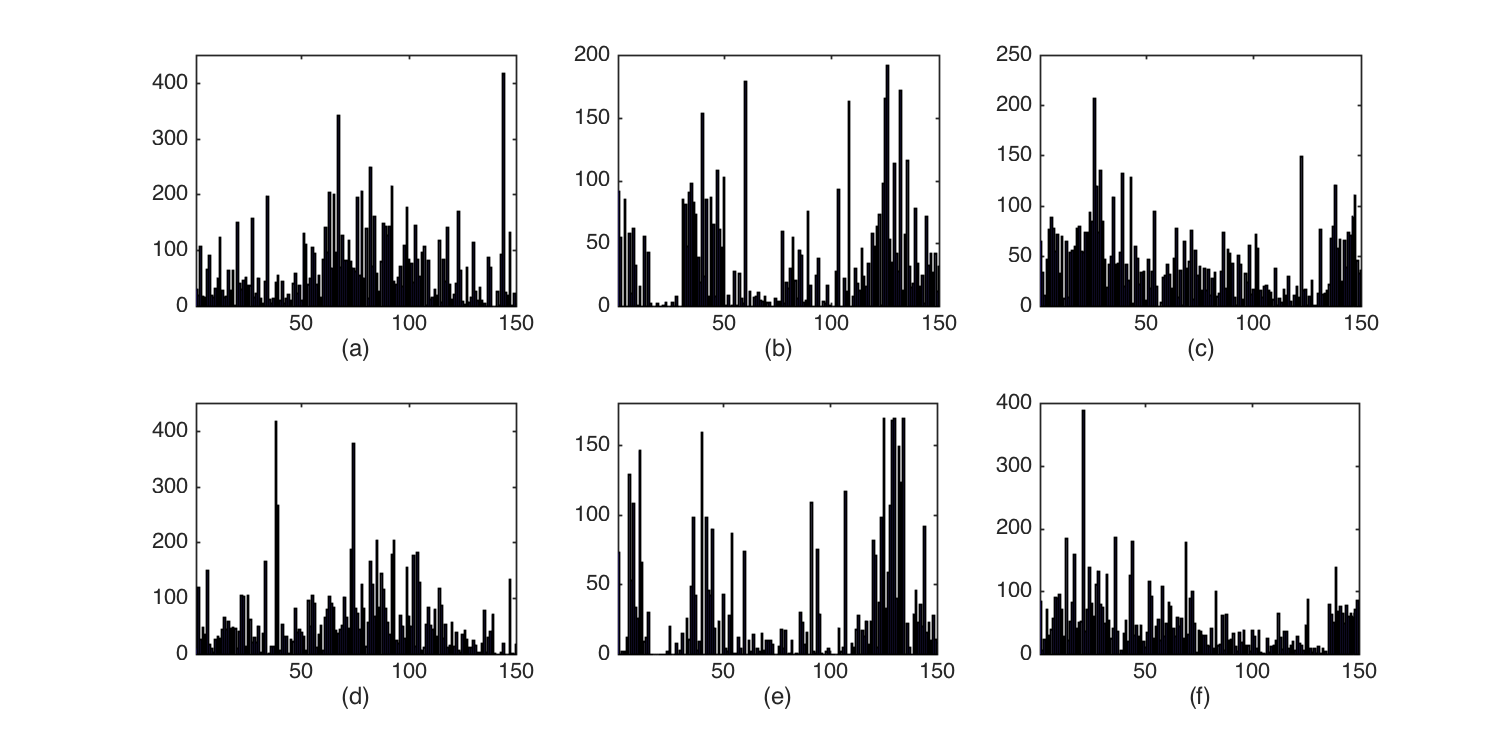
\includegraphics[width=1\linewidth]{q3_hist}
		\caption{Histogram of sample training images: (a), (b) \& (c) training images, (d), (e) \& (f)}
		\label{fig:q3_hist}
	\end{center}
\end{figure}



Figure~\ref{fig:q3_hist} shows the histogram of some example training and testing images. The recognition problem was transformed to a data point based classification problem, which was then solved by the multi-class SVM classification. The accuracy of recognition was affected by value of $K$ as shown in Figure~\ref{fig:q3_k}. The correction rate increased rapidly when the increasing $K$ was small. However, we also observed that the accuracy converged to maximum rate as $K$ reached around 50. The complexity of the SVM is dependent on the number of support vectors and the data dimension ($K$). Hence, it's optimum to set $M$ at 50 to 80 to avoid overcomplexity. 

\begin{figure}
	\begin{center}
		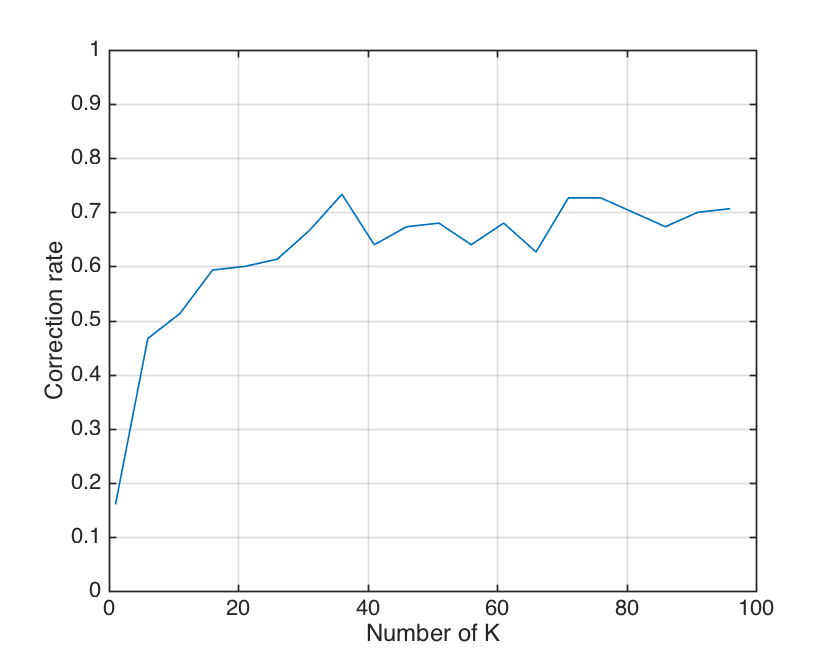
\includegraphics[width=0.8\linewidth]{q3_k}
		\caption{Accuracy affected by the number of K}
		\label{fig:q3_k}
	\end{center}
\end{figure}

\subsection{OVO and OVR}
The method of multi-class extension of binary SVMs could affect the accuracy of classification. To investigate this, we fixed the other parameters as: RBF kernel, $\sigma = 2^{15}$, $C = 2^{15}$ and $K = 50$, and tested both OVO and OVR extended SVMs. The correction rates were averaged over 10 iterations to reduce the variance. The resulting accuracy rates are shown in Table ~\ref{tab:ovr_ovo}, which states that the OVR method averagely has 2 \% accuracy more than OVO method.  \\

%\begin{table}[h!]
%	\centering
%	\caption{Accuracy of OVO and OVR}
%	\label{tab:ovr_ovo}
%	\begin{tabular}{ccc}
%		\toprule
%		Some & actual & content\\
%		\midrule
%		prettifies & the & content\\
%		as & well & as\\
%		using & the & booktabs package\\
%		\bottomrule
%	\end{tabular}
%\end{table}

\begin{table}[h!]
	\centering
	\caption{Comparing OVO and OVR}
	\label{tab:ovr_ovo}
	\begin{tabular}{ccc}
		\toprule
		~ & OVR & OVO\\
		\midrule
		Accuracy & 66.67\% & 64.27 \%\\
		\bottomrule
	\end{tabular}
\end{table}

\subsection{Kernel type}
In this coursework, we applied and compared two types of kernel functions: RBF function (Eq.\ref{eq:RBF}) and Polynomial kernel function
\begin{equation}
k(\boldsymbol{x}, \boldsymbol{x'}) = (\boldsymbol{x^T} \boldsymbol{x'} + c)^M
\label{eq:poly}
\end{equation}
where $M$ is the polynomial order. We trained the SVMs with two kernel functions separately and compared their performances. The RBF parameters $\sigma$ was set to \texttt{'auto'}, which enables the MATLAB function \texttt{fitcsvm} to automatically select an optimum value. The Polynomial order $M$ was set to 3. OVR extension was used for both kernel functions. The accuracy of such configuration is shown in Table.\ref{tab:rbf_poly}. The results can only suggest that the polynomial kernel function with this specific configuration yields better accuracy. However, the results were subjective to the parameters and more importantly, the data sets used. The two kernel functions generates different high dimensional kernel spaces, which should be optimum for different types of data sets.

\begin{table}[h!]
	\centering
	\caption{Comparing RBF and Polynomial kernel function}
	\label{tab:rbf_poly}
	\begin{tabular}{ccc}
		\toprule
		~ & RBF & Polynomial\\
		\midrule
		Accuracy & 63.82\% & 65.00 \%\\
		\bottomrule
	\end{tabular}
\end{table}

\subsection{Kernel parameter $\sigma$ and $C$}
Recall that in Question 2, the kernel parameter for RBF ($\sigma$) affected the overfitting and underfitting of the model, which affects the performance of the model with new testing data points. The parameter $C$ which controls the margin of each SVM also affect the generalization of the trained models. We trained and tested OVO extended SVMs and evaluated the correction rate varying the $\sigma$ from $2^{-5}$ to $2^{40}$ while varying the parameter $C$ from $2^{-20}$ to $2^{20}$. The result is visualized in Figure~\ref{fig:q3_ovo3D}. The accuracy for each parameter pair $\{\sigma, $C$ \}$ was averaged over 10 iterations. Figure~\ref{fig:q3_ovo3D} can be summarized as: 

\begin{itemize}
\item Increasing $C$ increased the accuracy when $C$ is below $2^5$. Further increasing $C$ did not increase the accuracy rate. However, higher value of $C$ may lead to overfitting if the model is to be tested by new testing data since it lead to smaller margin;
\item The accuracy has a peak with respect to $\sigma$ and reduces when $\sigma$ was large. This verified the theory that $\sigma$ could lead to overfitting and increasing of testing lost.
\end{itemize}

\begin{figure}
	\begin{center}
		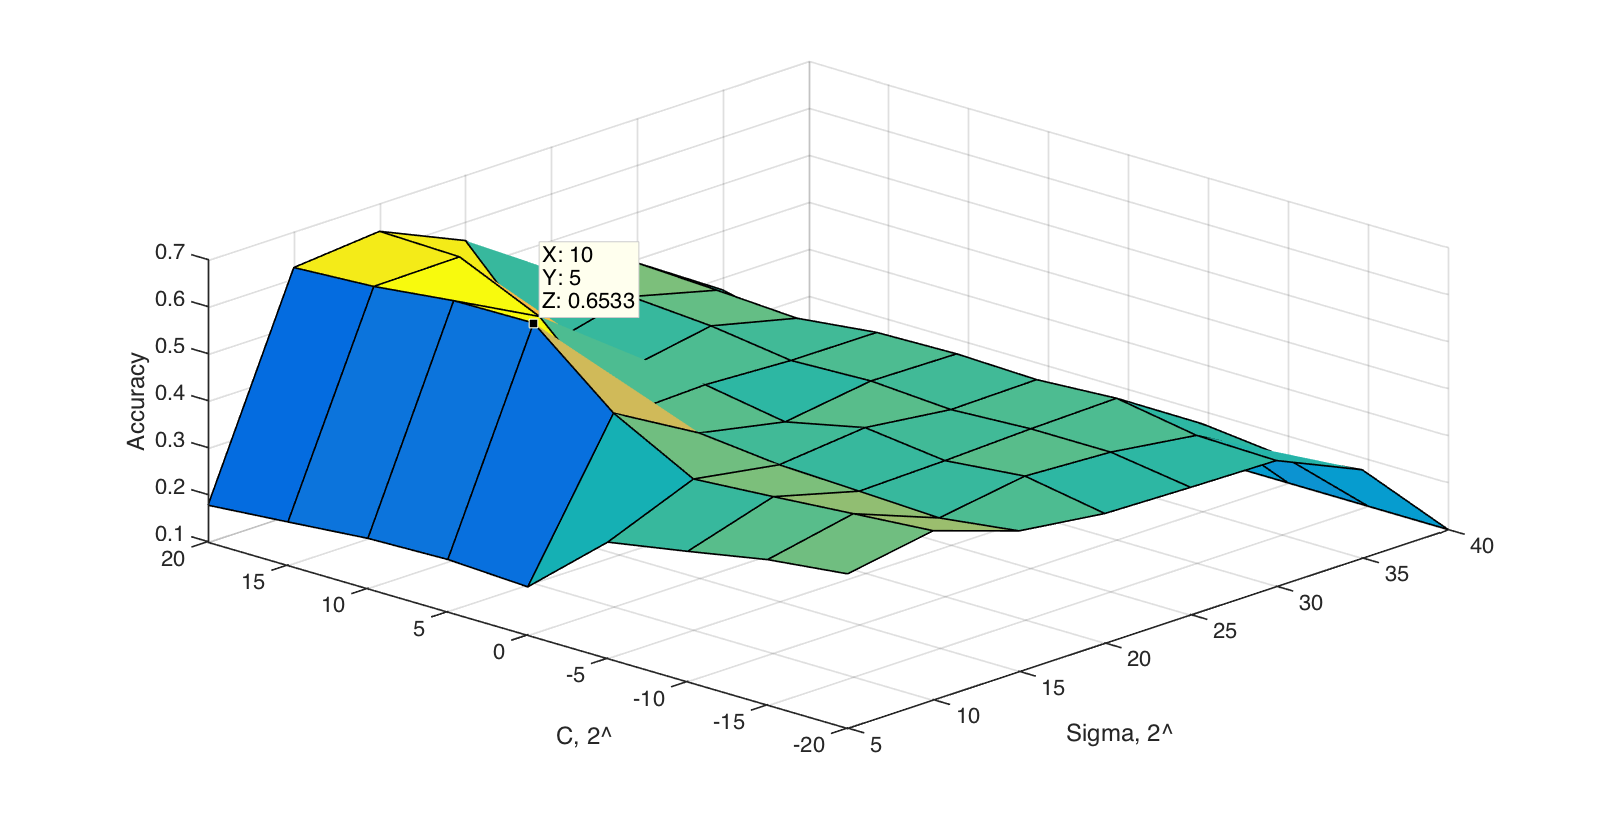
\includegraphics[width=1\linewidth]{q3_ovo3D}
		\caption{Accuracy varying both $\sigma$ and $C$}
		\label{fig:q3_ovo3D}
	\end{center}
\end{figure}


Figure~\ref{fig:q3_confmat} contains the confusion matrices for some combinations of $\{\sigma, C \}$, with (a) showing the result of the optimal pair of parameters, (b) and (c) showing less optimal results. It can be found that the class 3 and 4 were less well-classified when the overall accuracy was lower. 

\begin{figure}
	
	\begin{subfigure}[H]{0.3 \columnwidth}
		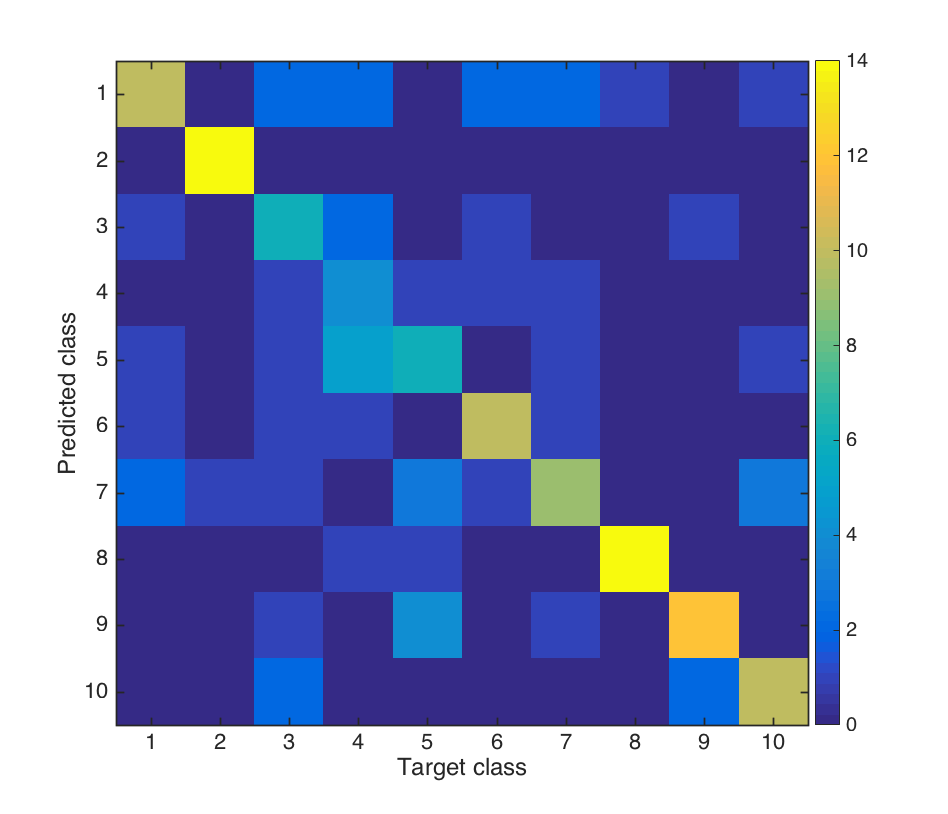
\includegraphics[width = 1\columnwidth]{q3_confmat1}\hfill
		\caption{$\sigma = 2^{10}$, \\$C = 2^5$}
	\end{subfigure}
	~
	\begin{subfigure}[H]{0.3 \columnwidth}
		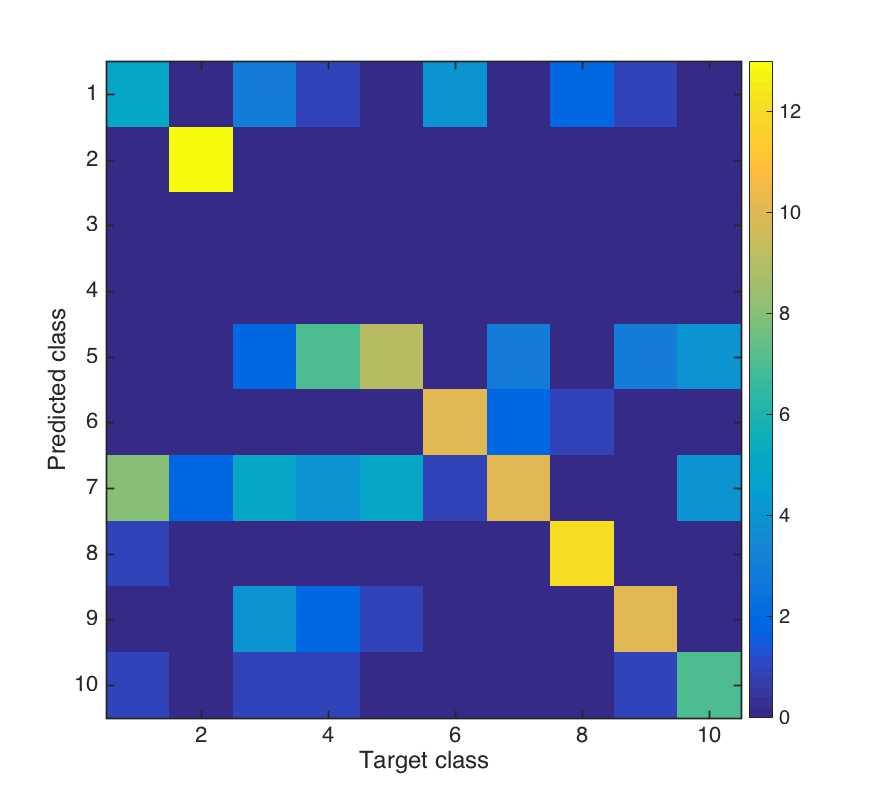
\includegraphics[width = 1\columnwidth]{q3_confmat2}
		\caption{$\sigma = 2^{10}$, \\$C = 2^0$}
	\end{subfigure}
	~
	\begin{subfigure}[H]{0.3 \columnwidth}
		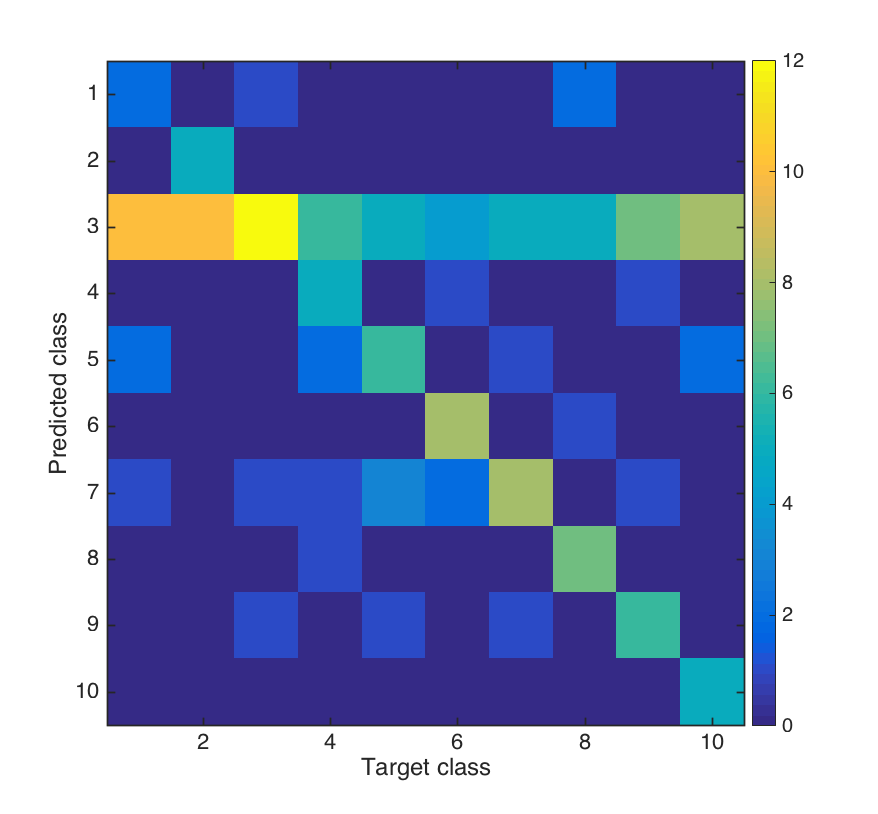
\includegraphics[width = 1\columnwidth]{q3_confmat3}
		\caption{$\sigma = 2^{7}$, \\$C = 2^5$}
	\end{subfigure}
		
	\caption{Confusion matrices}
	\label{fig:q3_confmat}
\end{figure}




{\small
\bibliographystyle{ieeetr}
\bibliography{egbib}
}

\onecolumn
\appendix
\section{Appendix 1 MATLAB Code}
\subsection{One vs Rest extension}
\lstinputlisting{fMSVM1vR.m}

\subsection{One vs one extension}
\lstinputlisting{fMSVM1v1.m}

\subsection{Bag of Words vector quantisation pr}
\lstinputlisting{getDataHQ.m}

\end{document}
